

\section{Preliminary Work}

As visualized in \reffig{fig:method}, two steps of this proposed methodology has already been carried out: A small-scale wasm application, and the basics of a browser-based visual programming language. These where both part of the preliminary work done in preparation of this thesis proposal. This chapter will elaborate upon these Works.


\subsection*{Wasm Application}

WebAssembly is a major component of this proposed thesis. However, the compilation target is still widely regarded as being "bleeding edge" (FIND SOURCE). This makes it all the more vital to gain some level of experience using the compile target before using it in more complicated scenario's. 

The Geomatics curriculum this thesis proposal is part of, offers a subject called "Research Assignment". This course offers students to gain experience in a geomatics-related topic of choice, and this made it the perfect context to try out WebAssembly for a geomatics web application.

The assignment given was to deliver a prototype for an online cityJSON validator. 
WebAssembly was to be used to perform a very fast JSON schema check over a user submitted json, among other things. 
This assignment was carried out successfully, and the delivered prototype (\reffig{fig:cjval-prototype}) played a role in the official CityJSON validator (\reffig{fig:cjval-official}), which uses WebAssembly. 

\begin{figure}[!tbp]
    \centering
    \begin{minipage}[b]{0.45\textwidth}
      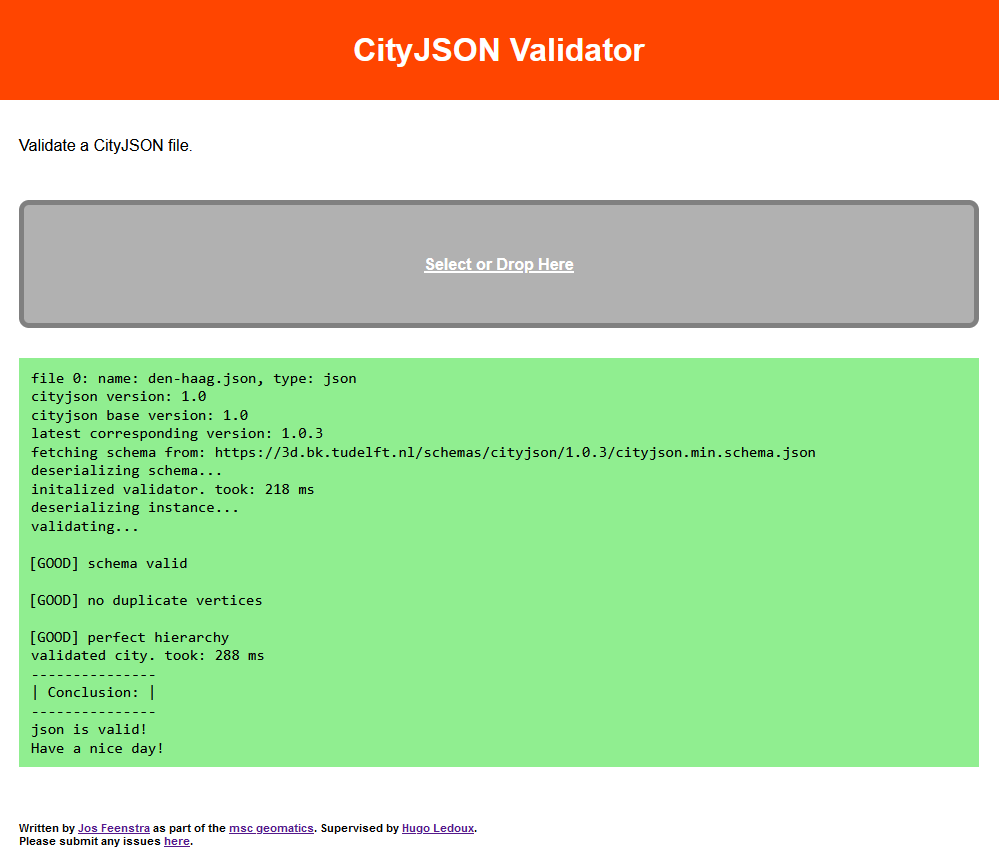
\includegraphics[width=\textwidth]{../images/cjval-prototype.PNG}
      \caption{The prototype}
      \label{fig:cjval-prototype}
    \end{minipage}
    \hfill
    \begin{minipage}[b]{0.45\textwidth}
      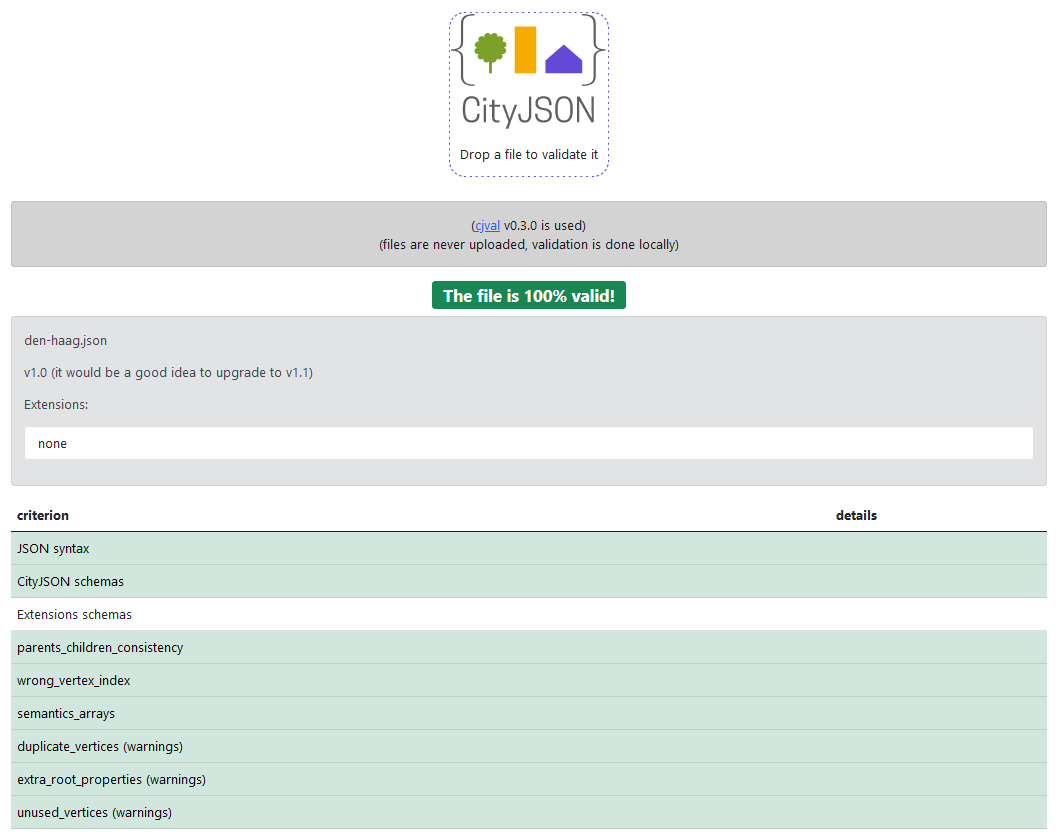
\includegraphics[width=\textwidth]{../images/cjval-official.PNG}
      \caption{The official validator}
      \label{fig:cjval-official}
    \end{minipage}
\end{figure}


Creating this application was very insightful. I would like to point out a few key insights, which will undoubtedly play an important role in the proposed thesis: 

\begin{itemize}

    \item The language this application was compiled from was Rust, not C++. Rust offers first-hand WebAssembly supports, as its default compiler supports WebAssembly. Surrounding tooling like \textit{wasm-pack} and community support \& tutorials made using WebAssembly within web applications very doable. 
    C++ will still be used in the proposed thesis for the sake of compiling existing libraries, but if the necessity arises to write custom WebAssembly components, Rust will be preferred, taking advantage of these aspects, and the fact that wasm can integrate multiple languages.

    \item It was very interesting to discover how WebAssembly supports a hybrid gui + cli setup. 
    The assignment was carried out by first developing a native Rust CLI-application which can be used as a standalone validator. 
    This code was then 'wrapped' as an api, and together with \textit{wasm-pack}, exposed and integrated within a website. 
    The advantage this offers is synergy between CLI and GUI. Any change made or feature added to the original application can easily be integrated within the web-exposed application. It also makes sure that a user can choose what interface they prefer. 

    % TODO diagram 

    \item The resulting application is extremely fast. It is one thing to theorize about performance gain, and another thing to experience it, and what it means for the usability of an application. The validation was often just as fast as the native binary application, and sometimes, for reasons not yet discovered, WebAssembly was even faster. When you start comparing this speed to other web-based json validators, this performance gain is even more apparent. A process which normally takes minutes now completes within a second. 

    % (TODO: maybe speed comparrison of https://jsonschemalint.com/#!/version/draft-07/markup/json
    % vs https://validator.cityjson.org/)



\end{itemize}







\subsection*{VPL Prototype}

The second component which was deemed 

Nodes 

Geon engine
